% CS670 - Reinforcement Learning
% Dynamic Programming Assignment
% Gabriel Dulac-Arnold <gabe@squirrelsoup.net>
% Johannes H. Jensen <johannj@stud.ntnu.no>
\documentclass[a4paper]{article}
%\usepackage{multicol}
\usepackage{graphicx}
\usepackage[top=2cm,nohead,nofoot]{geometry}
\graphicspath{{../graphs/}}

\author{Gabriel Dulac-Arnold $<$gabe@squirrelsoup.net$>$ (CS09F004) \\
Johannes H. Jensen $<$johannj@stud.ntnu.no$>$ (CS09F005)}
\title{CS670 - Reinforcement Learning \\
\emph{Dynamic Programming Assignment}}

\begin{document}
\setlength{\parskip}{2ex}
\maketitle

\section{Value Iteration}

Value iteration with $\theta=0.01$ produced the following value functions:

\begin{figure}[h]
\center
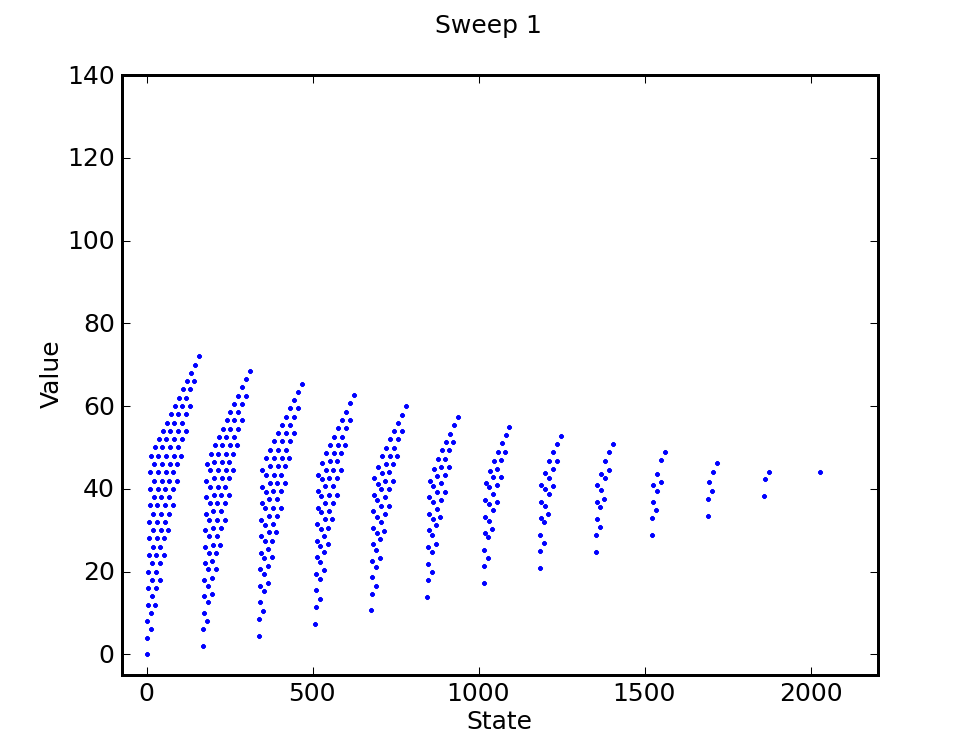
\includegraphics[scale=0.75]{value_iteration/sweep_1.png}
\caption{$V(s)$ after sweep 1}
\end{figure}

\begin{figure}[p]
\center
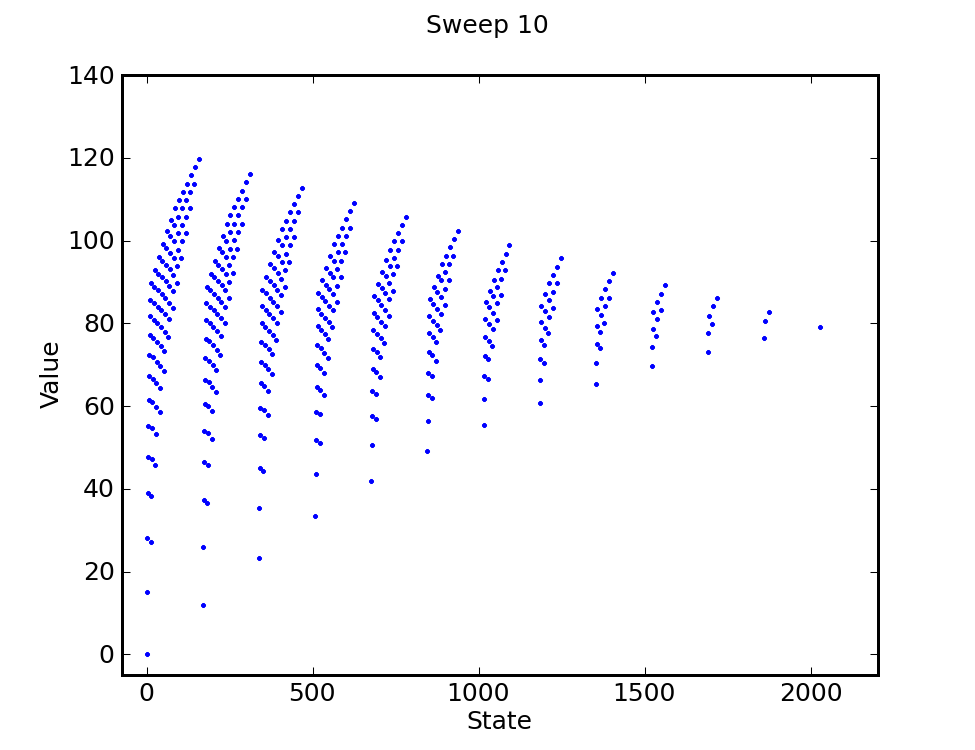
\includegraphics[scale=0.75]{value_iteration/sweep_10.png}
\caption{$V(s)$ after sweep 10}
\end{figure}

\begin{figure}[p]
\center
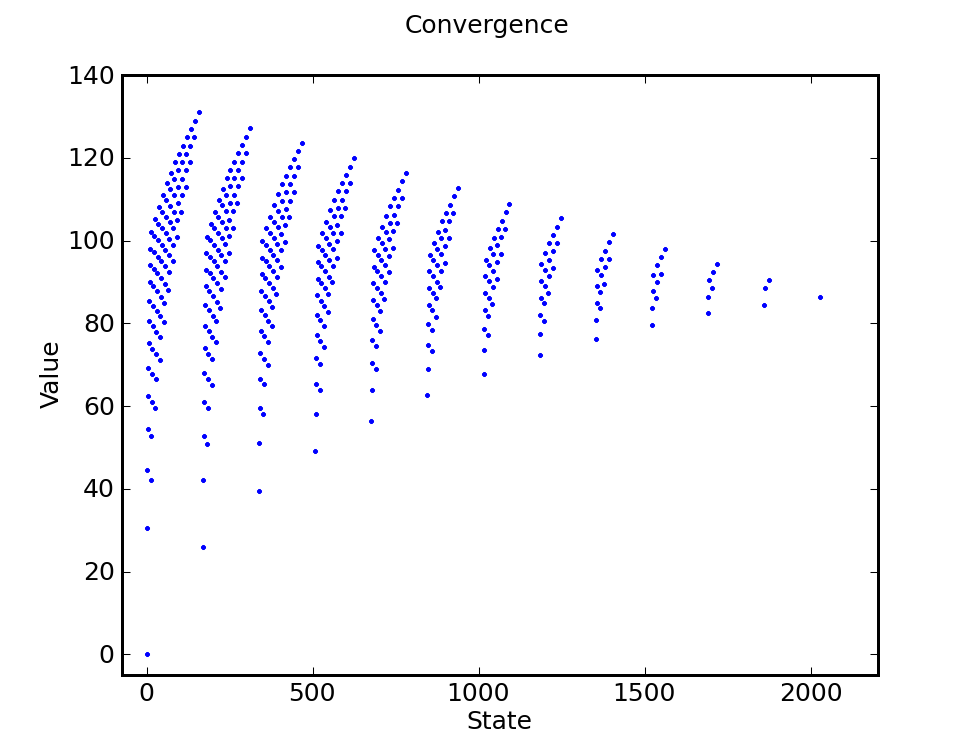
\includegraphics[scale=0.75]{value_iteration/convergence.png}
\caption{$V^*(s)$ at convergence}
\end{figure}


\newpage
\section{Policy Iteration}

Policy Iteration with $\theta=0.01$ gave an optimal policy and value function
after 4 policy evaluations:

\begin{figure}[h]
\center
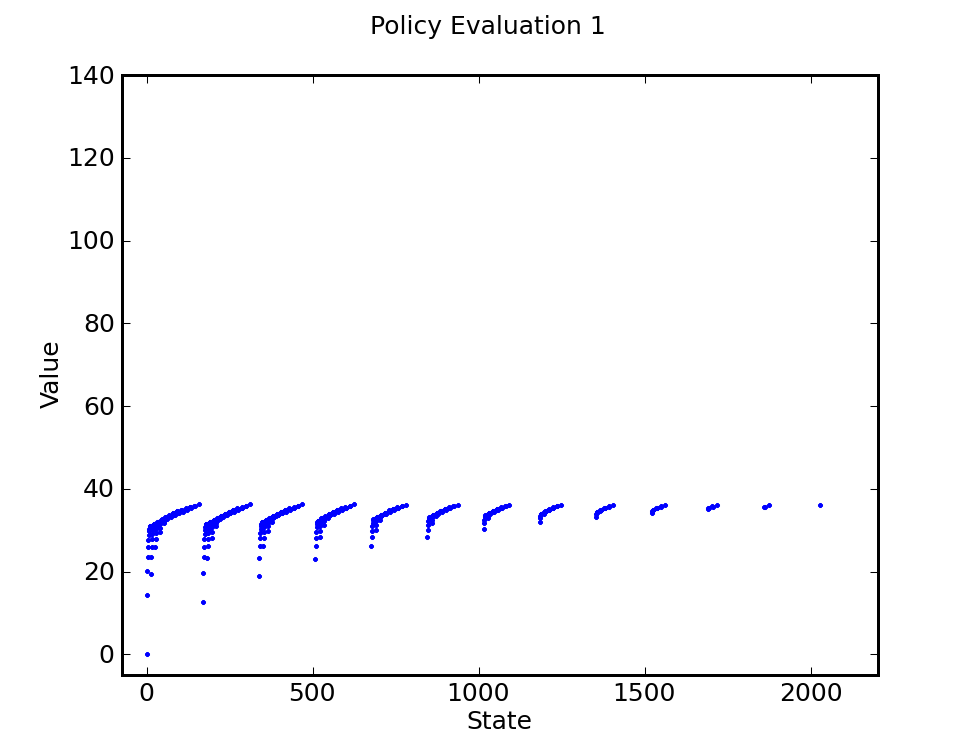
\includegraphics[scale=0.75]{policy_iteration/evaluation_1.png}
\caption{$V(s)$ after policy evaluation 1}
\end{figure}

\begin{figure}[h]
\center
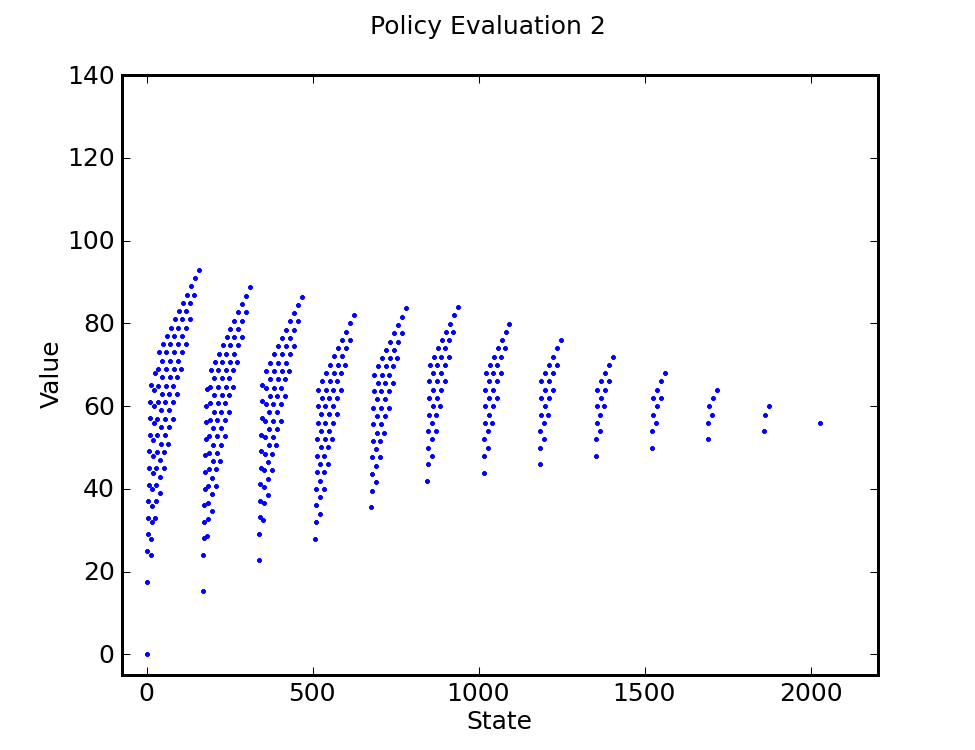
\includegraphics[scale=0.75]{policy_iteration/evaluation_2.png}
\caption{$V(s)$ after policy evaluation 2}
\end{figure}

\begin{figure}[h]
\center
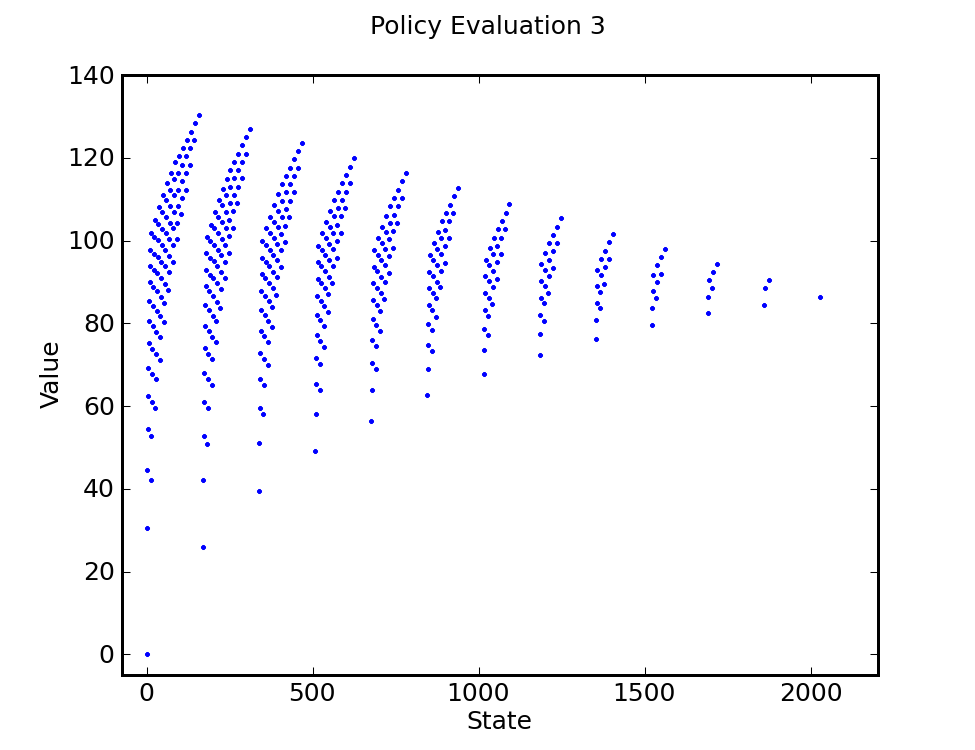
\includegraphics[scale=0.75]{policy_iteration/evaluation_3.png}
\caption{$V(s)$ after policy evaluation 3}
\end{figure}

\begin{figure}[h]
\center
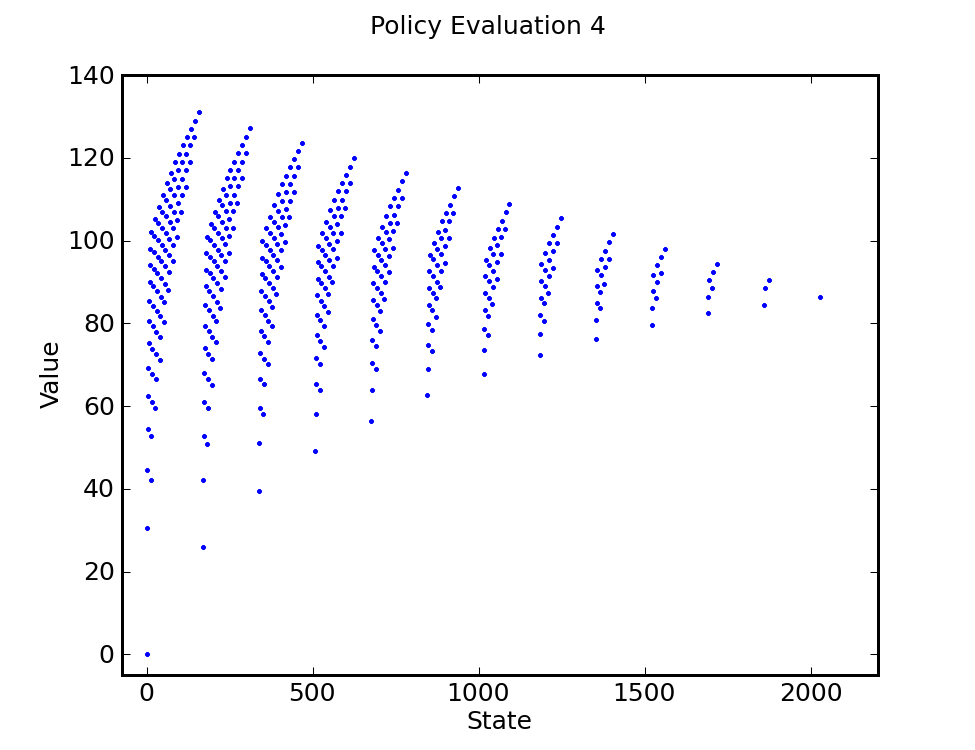
\includegraphics[scale=0.75]{policy_iteration/evaluation_4.png}
\caption{$V^*(s)$ after policy evaluation 4}
\end{figure}

\end{document}





